\chapter{Determining the Complex Relative Permittivity}


From worksheet ?? it is known that to find the complex relative permittivity, $\epsilon_0$, a set of at least six measurements are needed. Three with vertical polarization and three with horizontal polarization. So the first part of this worksheet will be about the performed measurement the next part will be data manipulation to find $\epsilon_0$ for both the gym and the parking lot.

\section{Measurement}
\subsection{Procedure}
\begin{enumerate}
	\item Decide frequency and incidence angle
	\item Decide measurement setup, including $P_t$ heights and distances between transmitter and receiver for all three measurements points
	\item Determine $G_t$, $G_r$, $L$, $\alpha_t$, $\alpha_r$ for both horizontal and vertical cases
	\item Calculate $\lambda$, k, $r_1$, $r_2$
	\item Measure $P_r$ in all six cases
	\item Find intersection point using \autoref{two-ray-circle} for both horizontal and vertical polarization
	\item Calculate the complex relative permittivity using \autoref{crp}
\end{enumerate}

\subsection{Setup}
So first it is decided to use both 858MHz and 2580MHz as frequencies as both of these are used in the extensive measurement campaign performed in the project. The incidence angle are chosen to 45 degree, based on the simplification of height distance relation. 
The setup used is the same as for the campaign and can be found in the measurement journal. Though only the patch antennas are used for this. The height and distances are calculated so the follows the description seen on \autoref{fig:measurepoints}. 

\begin{figure}[H]
\centering
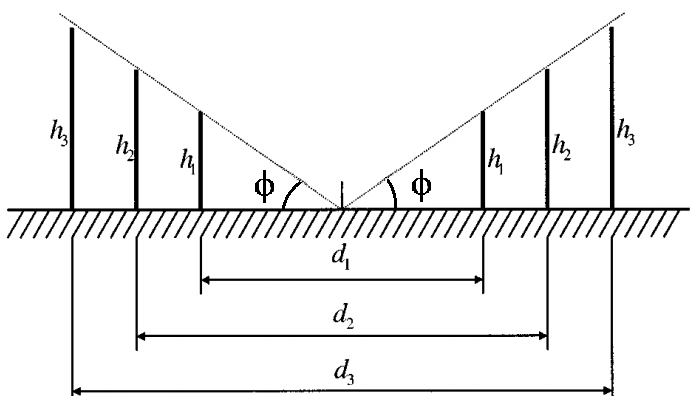
\includegraphics[width=0.6\textwidth]{figure/measurepoints.png}
\caption{Illustration of the three distances and heights needed. Figure taken from \citep{Kim}.}
\label{fig:measurepoints}
\end{figure}


\begin{table}[H]
\centering
\begin{tabular}{|c|c|c|c|}\hline
					&\textbf{Height}	&\textbf{Distance}	&\textbf{Power}	\\\hline
\textbf{Point 1}	&0.5m				&1m					&0dBm			\\\hline
\textbf{Point 2}	&1m					&2m					&0dBm			\\\hline
\textbf{Point 3}	&2m					&4m					&0dBm			\\\hline
\end{tabular}
\caption{Height distance for the different measurement points.}
\label{tab:height_distance}
\end{table}


\subsection{Pre-processing}
Based on a measurement performed in Satimo Starlab all gains for the antenna can be found. These are summarized in \autoref{tab:gains}
\begin{table}[H]
\centering
\begin{tabular}{|c|c|c|c|c|}\hline
\textbf{Frequency}		& \multicolumn{2}{c|}{\textbf{858 MHz}}&\multicolumn{2}{c|}{\textbf{2580 MHz}}		\\\hline
\textbf{Polarization}	& \textbf{Vertical}	&\textbf{Horizontal}	& \textbf{Vertical}	&\textbf{Horizontal}\\\hline		
\textbf{Gain angle 0}	&-3.5745 dB	&-3.6360 dB	&4.3624 dB	&4.3446 dB	\\\hline
\textbf{Gain angle 45}	&-4.8326 dB	&-6.9685 dB	&-2.6601 dB	&-3.5324 dB	\\\hline		
\end{tabular}
\caption{Gains for the patch antennas.}
\label{tab:gains}
\end{table} 

From the linkbudget worksheet it is found that L is 0.9 dB for 858 MHz and 1.6 dB for 2580 MHz.

The last parameters can then be calculated and are summarized in \autoref{tab:parameters}

\begin{table}[H]
\centering
\begin{tabular}{|c|c|c|}\hline
\textbf{Parameter}	&\textbf{Description}		&\textbf{Magnitude}	\\\hline
$\lambda_{858MHz}$	& Wavelength for 858 MHz				&0.3497 m			\\\hline
$\lambda_{2580MHz}$	& Wavelength for 2580 MHz				&0.1163 m			\\\hline
$k_{858MHz}$		& Wave number for 858 MHz				&17.9699			\\\hline
$k_{2580MHz}$		& Wave number for 2580 MHz				&54.0354			\\\hline
$r_{1,1}$			& Direct distance for point 1			&1 m				\\\hline
$r_{1,2}$			& Length of reflected path  for point 1	&$1\sqrt{2}$ m		\\\hline
$r_{2,1}$			& Direct distance  for point 2			&2 m				\\\hline
$r_{2,2}$			& Length of reflected path for point 2	&$2\sqrt{2}$ m		\\\hline
$r_{3,1}$			& Direct distance  for point 3			&4 m				\\\hline
$r_{3,2}$			& Length of reflected path for point 3	&$4\sqrt{2}$ m		\\\hline
\end{tabular}
\caption{Remaining parameters needed for calculation}
\label{tab:summarized}
\end{table}

\subsection{Measured data}

At the each measurement point is gathered 10 measurements and the means are shown in \autoref{tab:data}.

\begin{table}[H]
\centering
\label{my-label}
\begin{tabular}{|l|l|l|p{3.5cm}|p{3.5cm}|}
\hline
\textbf{Frequency} & \textbf{Polarization} & \textbf{Point} & \textbf{Power received in the gym} & \textbf{Power received on the parking lot} \\ \hline
858 MHz            & Horizontal            & 1              & -41,38		& -40,561		\\ \hline
858 MHz            & Horizontal            & 2              & -48,51		& -47,188		\\ \hline
858 MHz            & Horizontal            & 3              & -57,195 		& -53,858		\\ \hline
858 MHz            & Vertical              & 1              & -37,55 		& -38,7			\\ \hline
858 MHz            & Vertical              & 2              & -44,986		& -46,109		\\ \hline
858 MHz            & Vertical              & 3              & -51,463		& -50,34		\\ \hline
2580 MHz           & Horizontal            & 1              & -39,148		& -35,484		\\ \hline
2580 MHz           & Horizontal            & 2              & -45,63		& -43,502		\\ \hline
2580 MHz           & Horizontal            & 3              & -50,888		& -47,314		\\ \hline
2580 MHz           & Vertical              & 1              & -40,145		& -36,232		\\ \hline
2580 MHz           & Vertical              & 2              & -45,33		& -41,253		\\ \hline
2580 MHz           & Vertical              & 3              & -51,079		& -47,219		\\ \hline
\end{tabular}
\caption{Measured data}
\label{tab:data}
\end{table}

\subsection{Post-processing}
